\documentclass[border = 1cm, preview, varwidth=\maxdimen]{standalone}

\usepackage{xeCJK}

% mathematics
\usepackage{amsmath}

% tikz
\usepackage{tikz}
\usepackage{ifthen}
\usetikzlibrary{arrows}
\usetikzlibrary{automata}
\usetikzlibrary{positioning}
\tikzset{->, > = stealth', node distance = 1in}

\begin{document}
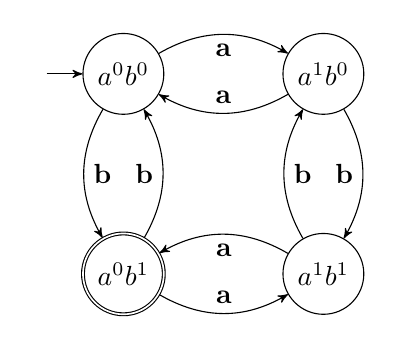
\begin{tikzpicture}
  % nodes
  \node [state, initial, initial text = ] (a0b0) {$a^0b^0$};
  \node [state, right of = a0b0] (a1b0) {$a^1b^0$};
  \node [state, accepting, below of = a0b0] (a0b1) {$a^0b^1$};
  \node [state, right of = a0b1] (a1b1) {$a^1b^1$};
  % paths
  \draw (a0b0) edge [bend right, right] node {\bf b} (a0b1);
  \draw (a0b1) edge [bend right, left] node {\bf b} (a0b0);
  \draw (a0b0) edge [bend left, below] node {\bf a} (a1b0);
  \draw (a1b0) edge [bend left, above] node {\bf a} (a0b0);
  \draw (a0b1) edge [bend right, above] node {\bf a} (a1b1);
  \draw (a1b1) edge [bend right, below] node {\bf a} (a0b1);
  \draw (a1b0) edge [bend left, left] node {\bf b} (a1b1);
  \draw (a1b1) edge [bend left, right] node {\bf b} (a1b0);
\end{tikzpicture}
\end{document}
